\chapter{拟合优度}
\label{ch:week3}
\section{简单回归的情形}
\sourcepage{3}{1}{3/1}
\label{sec:simple-properties}
本章区分拟合值与残差，并介绍判定系数 $R^2$。
\[y_i=\beta_0+\beta_1x_i+u_i,\qquad
\hat y_i=\hat\beta_0+\hat\beta_1x_i.\]
\begin{definition}[误差与残差]
\[\underbrace{u_i=y_i-\beta_0-\beta_1x_i}_{\text{总体误差}},\qquad
\underbrace{\hat u_i=y_i-\hat y_i=y_i-\hat\beta_0-\hat\beta_1x_i}_{\text{OLS 残差}}.\]
完成拟合后，残差可以计算并观测；总体误差则依赖未知的总体参数。
\end{definition}

\subsection{含截距 OLS 的三个样本性质}
\paragraph{性质一：残差的样本均值为零。}
OLS 使 $Q(b_0,b_1)=\sum_i(y_i-b_0-b_1x_i)^2$ 最小。在最优点，
\[\left.\frac{\partial Q}{\partial b_0}\right|_{\hat\beta}
=-2\sum_{i=1}^n\hat u_i=0
\quad\Longrightarrow\quad\hm{\sum_i\hat u_i=0},\quad\bar{\hat u}=0.\]

\paragraph{性质二：残差与 $x$ 在样本中正交。}
关于斜率的一阶条件为
\[\left.\frac{\partial Q}{\partial b_1}\right|_{\hat\beta}
=-2\sum_i x_i\hat u_i=0.\]
因此，
\begin{align*}
\Cov_n(x,\hat u)
&=\frac1n\sum_i(x_i-\bar x)(\hat u_i-\bar{\hat u})\\
&=\frac1n\left(\sum_i x_i\hat u_i-\bar x\sum_i\hat u_i\right)=0.
\end{align*}
\hy{残差与 $x$ 在样本中不相关}。若某个变量的方差为零，相关系数本身未定义；但正交关系仍成立。

每个观测可分解为 $y_i=\hat y_i+\hat u_i$，且拟合值与残差在样本中正交：
\[\sum_i\hat y_i\hat u_i
=\hat\beta_0\sum_i\hat u_i+\hat\beta_1\sum_i x_i\hat u_i=0.\]

\paragraph{总体矩条件：另一个层面的结论。}
总体矩条件可以利用迭代期望法则得到。若 $\E[u\mid x]=0$ 且所需可积性条件成立，则
\[\E[u]=\E\{\E[u\mid x]\}=0,\qquad
\E[xu]=\E\{x\E[u\mid x]\}=0.\]
\red{这些总体限制不能用来证明样本正规方程。}即使总体外生性假设不成立，上述样本恒等式仍直接来自残差平方和的最小化。\corr{sample-population}

\paragraph{性质三：样本均值点位于拟合线上。}
由于 $\hat\beta_0=\bar y-\hat\beta_1\bar x$，有
\[\hm{\bar y=\hat\beta_0+\hat\beta_1\bar x}.\]
也可以对 $\hat y_i=\hat\beta_0+\hat\beta_1x_i$ 取样本平均：
\[\bar{\hat y}=\frac1n\sum_i\hat y_i=\hat\beta_0+\hat\beta_1\bar x,
\qquad\bar y=\bar{\hat y}+\bar{\hat u}=\bar{\hat y}.\]
对应的\emph{总体}结论是：若 $\E[u]=0$，则 $\E[y]=\beta_0+\beta_1\E[x]$。这里应使用总体参数，而不是带帽的拟合系数。\corr{sample-population}

\section{平方和与拟合优度}
\sourcepage{3}{2}{3/2}
\label{sec:ss-decomposition}
\begin{definition}[总平方和、解释平方和与残差平方和]
\begin{align}
\TSS&=\sum_{i=1}^n(y_i-\bar y)^2=(n-1)s_y^2,\label{eq:tss}\\
\ESS&=\sum_{i=1}^n(\hat y_i-\bar y)^2,\label{eq:ess}\\
\RSS&=\sum_{i=1}^n\hat u_i^2=\sum_{i=1}^n(y_i-\hat y_i)^2.\label{eq:rss}
\end{align}
其中，$s_y^2=\sum_i(y_i-\bar y)^2/(n-1)$ 为样本方差。
\end{definition}
\blue{TSS：$y$ 围绕均值的总波动；ESS：回归线所解释的波动；RSS：回归未解释的残差波动。}本笔记用 ESS 表示\emph{解释}平方和；其他教材有时采用不同的缩写约定。

\begin{theorem}[平方和分解]
对于含截距的 OLS，
\begin{equation}\label{eq:anova}
\hm{\TSS=\ESS+\RSS}.
\end{equation}
\end{theorem}
\begin{proof}
由于 $y_i-\bar y=(\hat y_i-\bar y)+\hat u_i$，有
\begin{align*}
\TSS
&=\sum_i\bigl[(\hat y_i-\bar y)+\hat u_i\bigr]^2\\
&=\sum_i(\hat y_i-\bar y)^2+\sum_i\hat u_i^2
  +2\sum_i\hat u_i(\hat y_i-\bar y).
\end{align*}
因为 $\sum_i\hat u_i\hat y_i=0$ 且 $\sum_i\hat u_i=0$，交叉项为零，故式 \eqref{eq:anova} 成立。
\end{proof}
\blue{OLS 的目标是使 $\sum_i\hat u_i^2$ 最小，而不是使 $\sum_i\hat u_i$ 最小；后者为零来自截距的一阶条件。}

\subsection[判定系数的定义与解释]{判定系数 $R^2$ 的定义与解释}
当 $\TSS>0$ 时，定义
\begin{equation}\label{eq:r2}
\hm{R^2=\frac{\ESS}{\TSS}=1-\frac{\RSS}{\TSS}\in[0,1]}.
\end{equation}
\textbf{解释。}$R^2$ 衡量回归中各变量所解释的 \hy{$y$ 的样本波动占比}。例如，$R^2=0.85$ 表示因变量样本波动的 $85\%$ 可以由该回归解释。

若所有观测点都位于拟合线上，即 $y_i=\hat y_i$，则 $\RSS=0$、$\TSS=\ESS$，并且 $R^2=1$。这就是完全拟合。
\begin{figure}[htbp]
\centering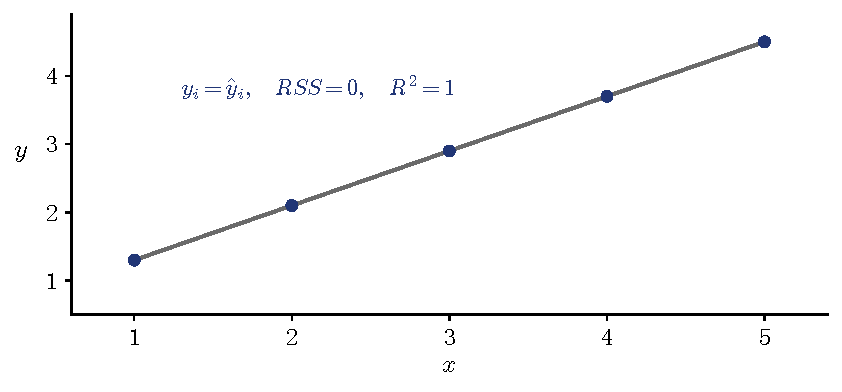
\includegraphics[width=.68\linewidth]{perfect_fit.pdf}
\caption{原稿中的完全拟合情形：全部示意观测点均落在拟合线上。}
\label{fig:perfect-fit}
\end{figure}

\subsection{相关系数平方的解释}
若 $y$ 与 $\hat y$ 的样本方差均为正，则
\begin{equation}\label{eq:r2-correlation}
R^2=\Corr_n(y,\hat y)^2
=\frac{\left[\sum_i(y_i-\bar y)(\hat y_i-\bar y)\right]^2}
{\left[\sum_i(y_i-\bar y)^2\right]\left[\sum_i(\hat y_i-\bar y)^2\right]}.
\end{equation}
利用 $y_i=\hat y_i+\hat u_i$、$\bar y=\bar{\hat y}$ 以及样本正交性，可得
\[\Cov_n(y,\hat y)=\Var_n(\hat y),\qquad
\Corr_n(y,\hat y)^2=\frac{\Var_n(\hat y)}{\Var_n(y)}=\frac{\ESS}{\TSS}.
\]
\added{若所有 $y_i$ 都相同，则 TSS 为零，此处的中心化 $R^2$ 未定义。若 $\hat y$ 为常数而 $y$ 存在变异，则 $R^2=0$，但 $\Corr_n(y,\hat y)$ 未定义；此时不能使用相关系数平方的公式进行计算。}\corr{r2-degenerate}

\subsection{图形比较}
\sourcepage{3}{3}{3/3}
\begin{figure}[htbp]
\centering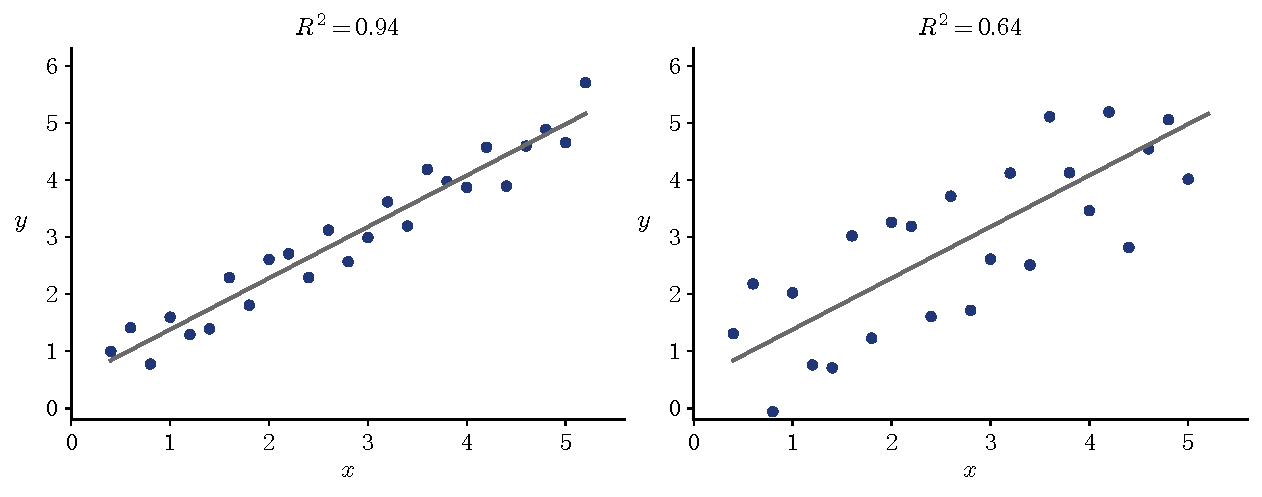
\includegraphics[width=.95\linewidth]{r_squared_comparison.pdf}
\caption{采用原稿中 $R^2=0.94$ 与 $R^2=0.64$ 的两组示意样本。图中的数值由新生成的观测点及其拟合线实际计算。}
\label{fig:r2-comparison}
\end{figure}
较高的 $R^2$ 对应较小的残差\emph{占比} $\RSS/\TSS$；较低的 $R^2$ 则对应较大的残差占比。\blue{较低时，仅靠当前回归变量，对 $y$ 的样本波动解释得较少。}不能只凭 $R^2$，就跨不同样本或不同因变量单位比较 RSS 的绝对大小。\corr{r2-rss}

\section{多元回归的情形}
\label{sec:multiple-properties}
模型、拟合值与残差分别为
\begin{align*}
y_i&=\beta_0+\beta_1x_{1i}+\cdots+\beta_kx_{ki}+u_i,\\
\hat y_i&=\hat\beta_0+\hat\beta_1x_{1i}+\cdots+\hat\beta_kx_{ki},\\
\hat u_i&=y_i-\hat y_i.
\end{align*}
前述三个样本性质可推广到多元回归。

\paragraph{性质一：残差均值为零。}
令 $Q(b)=\sum_i(y_i-b_0-\sum_{j=1}^k b_jx_{ji})^2$，则
\[\left.\frac{\partial Q}{\partial b_0}\right|_{\hat\beta}
=-2\sum_i\hat u_i=0
\quad\Longrightarrow\quad\sum_i\hat u_i=0,\quad\bar{\hat u}=0.\]

\paragraph{性质二：残差与每个已纳入的回归变量在样本中正交。}
对于每个 $j=1,\ldots,k$，
\[\left.\frac{\partial Q}{\partial b_j}\right|_{\hat\beta}
=-2\sum_i x_{ji}\hat u_i=0
\quad\Longrightarrow\quad\hm{\sum_i x_{ji}\hat u_i=0}.\]
结合截距的一阶条件，得到 $\Cov_n(x_j,\hat u)=0$。

\paragraph{性质三：样本均值向量位于拟合超平面上。}
对 $y_i=\hat y_i+\hat u_i$ 取平均，得 $\bar y=\bar{\hat y}$，因此
\begin{align*}
\bar y
&=\frac1n\sum_i\left(\hat\beta_0+\hat\beta_1x_{1i}+\cdots+\hat\beta_kx_{ki}\right)\\
&=\hm{\hat\beta_0+\hat\beta_1\bar x_1+\cdots+\hat\beta_k\bar x_k}.
\end{align*}
采用与式 \eqref{eq:anova} 相同的证明，可知含截距的多元 OLS 仍满足 TSS $=$ ESS $+$ RSS，并适用同一个 $R^2$ 公式。

\section[增加回归变量与调整判定系数]{增加回归变量与调整 $R^2$}
\sourcepage{3}{4}{3/4}
\label{sec:adjusted-r2}
回顾以下定义：
\[\TSS=\sum_i(y_i-\bar y)^2,\quad
\ESS=\sum_i(\hat y_i-\bar y)^2,\quad
\RSS=\sum_i(y_i-\hat y_i)^2.\]
若增加回归变量，$R^2$ 会怎样变化？
\begin{itemize}
\item 对于\emph{相同观测和同一因变量}，若两个嵌套模型均含截距，新模型最小化后的 RSS 不会大于旧模型：将新增系数设为零，就可以复现旧模型的拟合。
\item 因此，$R^2$ \hy{不会下降}，但可能完全不变。不断加入变量可能导致样本内过拟合。\corr{r2-monotonic}
\item $R^2$ 不能建立因果关系。高 $R^2$ 不一定意味着因果，低 $R^2$ 也不能排除因果。
\end{itemize}

\subsection{自由度调整}
若不计截距有 $k$ 个回归变量，且 $n>k+1$、$\TSS>0$，则
\begin{equation}\label{eq:adjusted-r2}
\hm{\bar R^2=1-\frac{\RSS/(n-k-1)}{\TSS/(n-1)}
=1-\frac{n-1}{n-k-1}(1-R^2)}.
\end{equation}
\blue{自由度修正：增加回归变量会受到惩罚，RSS 的减少必须足以补偿损失的自由度。}
\begin{itemize}
\item $\bar R^2$ 对回归变量个数施加惩罚，因此增加变量时可能下降。
\item 若残差均方超过仅含均值模型的基准均方，它可以为负。
\item $\bar R^2$ 上升，只说明在此调整标准下，样本内拟合改善足够大；这并不证明变量具有实质重要性或因果作用。
\end{itemize}
\added{增加 $q$ 个回归变量时，$\bar R^2$ 上升当且仅当
\[
\frac{(\RSS_{\text{旧}}-\RSS_{\text{新}})/q}{\RSS_{\text{新}}/(n-k_{\text{新}}-1)}>1,
\]
其中假设分母为正。这是描述性的偏 $F$ 统计量门槛 1，并非常规显著性检验的临界值。}\corr{adjusted-meaning}

\begin{example}[平均绩点：原稿中的取舍]
使用原稿给出的舍入数值，且 $n=141$：
\begin{align*}
\text{仅含高中绩点：}\quad &R^2=0.172,\quad k=1,\\
&\bar R^2=1-\frac{140}{139}(1-0.172)=0.166043\ldots,\\
\text{高中绩点与 ACT：}\quad &R^2=0.176,\quad k=2,\\
&\bar R^2=1-\frac{140}{138}(1-0.176)=0.164058\ldots.
\end{align*}
加入 ACT 后，普通 $R^2$ 上升，而调整 $R^2$ 略微下降。这些结果由原稿中经过舍入的输入数值计算；超出输入精度的小数位仅表示算术计算精度。
\end{example}

\paragraph{注意（保留原稿的三点提醒）.}
\begin{enumerate}
\item $R^2$ 描述样本拟合：高 $R^2\ne$ 因果，低 $R^2\ne$ 没有因果。
\item 加入变量可能造成过拟合；调整 $R^2$ 虽引入惩罚，却不能单独保证样本外表现。
\item 良好的拟合并不自动消除遗漏变量偏误。
\end{enumerate}


\section{过原点回归与去均值}
\sourcepage{3}{5}{3/5}
\label{sec:rto}
回顾\emph{仅含截距}的回归：$\hat\beta_0=\bar y$，证明见下文。这一恒等式不适用于任意含 $x$ 的回归。

\subsection{过原点回归（RTO）}
有时模型被限制为经过原点。例如，某个生产关系假定投入为零时，期望产出也为零。这是额外的建模限制，并不是生产数据自动具备的性质。
\[y_i=\beta_1^{\rm RTO}x_i+u_i,\qquad
\hat y_i=\check\beta_1x_i,\qquad\check u_i=y_i-\hat y_i.\]
此处使用倒帽记号，区分这一拟合斜率及其残差与含截距 OLS 的对应量。最小化
\[Q(b_1)=\sum_i(y_i-b_1x_i)^2\]
可得一阶条件
\[\sum_i x_i(y_i-\check\beta_1x_i)=0
\quad\Longrightarrow\quad
\hm{\check\beta_1=\frac{\sum_i x_iy_i}{\sum_i x_i^2}}
\quad\text{其中 }\sum_i x_i^2>0.
\]

\subsection{去均值后可复现含截距回归的斜率}
定义 $A_i=y_i-\bar y$、$B_i=x_i-\bar x$。将 $A_i$ 对 $B_i$ 作过原点回归，其斜率为
\[\frac{\sum_iB_iA_i}{\sum_iB_i^2}
=\frac{\sum_i(x_i-\bar x)(y_i-\bar y)}{\sum_i(x_i-\bar x)^2}
=\hat\beta_1.\]
因此，对\emph{去均值}变量作无截距回归，可以复现普通\emph{含截距} OLS 的斜率。这不意味着未经中心化的无截距回归也具有相同斜率。\corr{demeaning}

对于含截距的 OLS，
\[y_i-\bar y=\hat\beta_1(x_i-\bar x)+\hat u_i.\]
\blue{截距项使回归线经过样本均值 $(\bar x,\bar y)$；去均值相当于平移坐标，不改变斜率。}
\begin{figure}[htbp]
\centering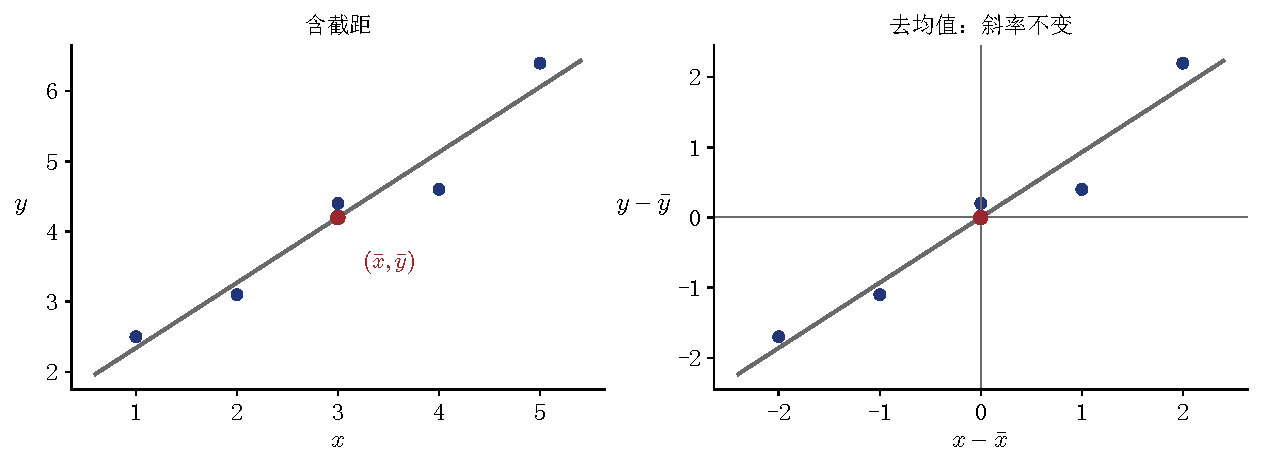
\includegraphics[width=.95\linewidth]{demeaning.pdf}
\caption{去均值将样本均值点移到原点，同时保留拟合斜率。本图采用示意观测。}
\label{fig:demeaning}
\end{figure}

\paragraph{原稿页底重复的例式（保留可见内容）.}
扫描页底再次写出了例式
\[\wage=\beta_0+\beta_1\educ+u,\]
并列出智力、家庭背景、经验和培训等未观测因素。它们仍与第 2 周的外生性讨论相关。此处不推测扫描可见范围之外的后续内容。

\subsection{OLS 公式：按补充推导页再次保留}
\sourcepage{3}{6}{补充推导页}
含截距时，
\[\hat\beta_1=\frac{\sum_i(x_i-\bar x)(y_i-\bar y)}{\sum_i(x_i-\bar x)^2},
\qquad\hat\beta_0=\bar y-\hat\beta_1\bar x.\]
不含截距时，
\begin{align*}
\frac{d}{db_1}\sum_i(y_i-b_1x_i)^2&=-2\sum_i x_i(y_i-b_1x_i),\\
\sum_i x_iy_i-\check\beta_1\sum_i x_i^2&=0,\\
\check\beta_1&=\frac{\sum_i x_iy_i}{\sum_i x_i^2}.
\end{align*}

\paragraph{为什么去均值有效？}
令 $x_i^*=x_i-\bar x$、$y_i^*=y_i-\bar y$，将 $y_i^*$ 对 $x_i^*$ 作无截距回归：
\[\hat\gamma=\frac{\sum_i x_i^*y_i^*}{\sum_i(x_i^*)^2}
=\frac{\sum_i(x_i-\bar x)(y_i-\bar y)}{\sum_i(x_i-\bar x)^2}=\hat\beta_1.\]
因此，就斜率而言，含截距 OLS $\Longleftrightarrow$ 去均值后的无截距 OLS。样本均值点变为 $(0,0)$，拟合线不发生旋转。

\paragraph{去均值就是对常数项回归后取残差。}
在仅含截距的回归 $y_i=b_0+e_i$ 中，
\[\frac{d}{db_0}\sum_i(y_i-b_0)^2=-2\sum_i(y_i-b_0)=0
\quad\Longrightarrow\quad\hat b_0=\bar y.\]
残差为 $y_i-\bar y$。同理，将 $x_i$ 对常数项回归，得到残差 $x_i-\bar x$。

\subsection{剔除线性影响：FWL 定理}
\label{sec:fwl-week3}
对于 $y_i=\beta_0+\beta_1x_i+\beta_2z_i+u_i$，原稿给出的三个步骤为：
\begin{enumerate}
\item 将 $y$ 对 $(1,z)$ 回归，得到残差 $r_{yi}$。
\item 将 $x$ 对 $(1,z)$ 回归，得到残差 $r_{xi}$。
\item 将 $r_y$ 对 $r_x$ 作无截距回归。
\end{enumerate}
结果为
\[\hm{\hat\beta_1=\frac{\sum_i r_{xi}r_{yi}}{\sum_i r_{xi}^2}}.\]
去均值是上述方法的一个特例：被剔除影响的变量只有常数项。这保留了原稿对两种方法之间联系的说明。

\section{无截距 OLS 的性质}
\sourcepage{3}{7}{3/6}
\label{sec:rto-properties}
回到过原点回归的目标函数，以及唯一系数对应的一阶条件：
\[\min_{b_1}\sum_i(y_i-b_1x_i)^2,\qquad
-2\sum_i x_i(y_i-\check\beta_1x_i)=0
\quad\Longrightarrow\quad\sum_i x_i\check u_i=0.\]
模型没有截距系数，因此也没有对截距求导的一阶条件。

\paragraph{性质一：残差均值不一定为零。}
模型不再强制 $\sum_i\check u_i=0$。某些特殊样本中它可以成立，但并无一般保证。

\paragraph{性质二：正交性仍成立，但协方差未必为零。}
仍有 $\sum_i x_i\check u_i=0$。然而，
\[\Cov_n(x,\check u)=\frac1n\sum_i x_i\check u_i-\bar x\bar{\check u}
=-\bar x\bar{\check u},\]
这一协方差一般不为零。\red{不能在无截距时把“内积为零”直接写成“样本不相关”。}\corr{rto-covariance}

\paragraph{性质三：样本均值点未必位于拟合线上。}
对 $y_i=\check\beta_1x_i+\check u_i$ 取平均，得
\[\bar y=\check\beta_1\bar x+\bar{\check u}.\]
因此，$\bar y=\check\beta_1\bar x$ 一般不成立。含截距时则由 $\bar{\hat u}=0$ 得到 $\bar y=\bar{\hat y}$。

\subsection[中心化判定系数可能为负]{中心化 $R^2$ 可能为负}
沿用 TSS 与 ESS 的中心化定义，有
\begin{equation}\label{eq:rto-cross-term}
\TSS=\ESS+\RSS+2\sum_i\check u_i(\hat y_i-\bar y).
\end{equation}
对于过原点拟合，$\sum_i\check u_i\hat y_i=0$，但 $\sum_i\check u_i$ 未必为零，因此交叉项不一定消失。\corr{rto-cross-term}
中心化统计量
\[R_c^2=1-\frac{\RSS}{\TSS}\]
可以为负：这意味着按平方误差衡量，强制过原点的拟合线比仅含均值的水平线 $\bar y$ 拟合得更差。
\begin{figure}[H]
\centering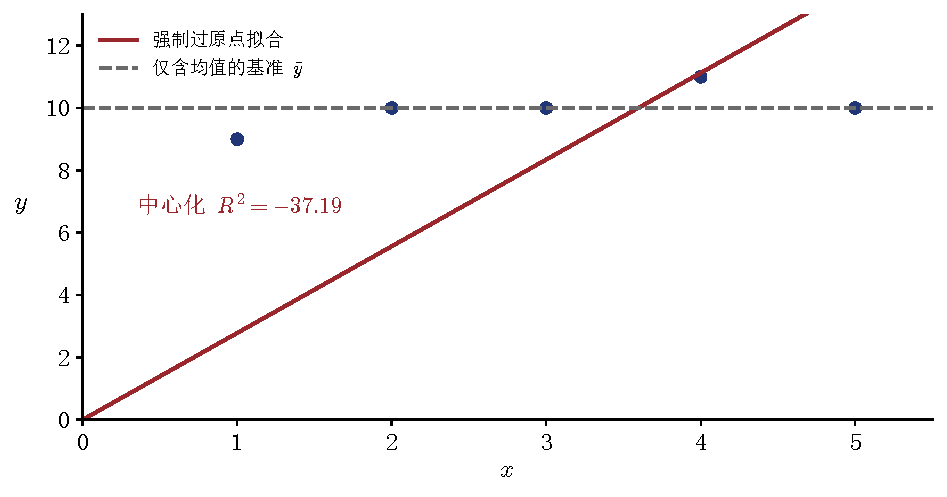
\includegraphics[width=.8\linewidth]{through_origin_negative_r2.pdf}
\caption{过原点拟合差于仅含均值的基准。示意数据 $x=(1,2,3,4,5)$、$y=(9,10,10,11,10)$ 产生了图中实际计算的负中心化 $R^2$。}
\label{fig:negative-r2}
\end{figure}
\added{某些软件对无截距模型报告\emph{非中心化}统计量 $R_u^2=1-\RSS/\sum_i y_i^2$。它以零为基准，而不是以 $\bar y$ 为基准，因此不能与含截距模型通常采用的中心化 $R^2$ 直接比较。}\corr{rto-r2}

\subsection*{本章小结}
\addcontentsline{toc}{subsection}{本章小结}
\begin{itemize}
\item 含截距时，OLS 残差的均值为零，与已纳入的回归变量在样本中正交，并有 TSS $=$ ESS $+$ RSS。
\item 在相同数据上对嵌套模型增加回归变量，普通 $R^2$ 不会下降，但调整 $R^2$ 可以下降。
\item 去均值与 FWL 保留完整模型中相应的斜率。省略截距会改变均值、协方差和中心化 $R^2$ 的性质。
\end{itemize}
